\section{Theorie}
\label{sec:Theorie}

Ziel des Versuches ist es, durch Absorptionskurven von $\beta$- und $\gamma$-Strahlung 
die Maximalenergie des Strahlers bzw. die Absoptionskoeffizienten von verschiedenen
Materialen zu bestimmen.\\

Trifft energetische Strahlung auf Materie, finden dabei Wechselwirkungen statt, die 
von der Art der Strahlung und deren Energie abhängen und letztendlich zu einer
Intensitätsabnahme führen. Im Folgenden wird die Materieschicht als Absorber bezeichnet.
Diese Abnahme der Intensität steigt dabei mit Anzahl der Wechselwirkungen.
Ein Maß für die Häufigkeit der Wechselwirkungen stellt der Wirkungsquerschnitt $\sigma$
dar. Er stellt eine fiktive Fläche dar, die ein Partikel des Absorbers haben müsste,
damit jedes Teilchen, das diese Fläche trifft, eine Wechselwirkung verursacht. $\sigma$
beschreibt demnach eine Wahrscheinlichkeit dafür, dass eine Wechselwirkung zwischen
Absorber und Teilchen stattfindet. \\
Für einen idealen Absorber der Dicke $D$, des Querschnitts $F$ und der Teilchendichte
$n$ pro Volumeneinheit, gibt 

\begin{equation*}
W = \frac{nFD\sigma}{F} = nD\sigma 
\end{equation*}

die beschriebene Wahrscheinlichkeit an. Die Wechselwirkung pro Zeiteinheit 
ist damit durch

\begin{equation*}
N = N_0 n D
\end{equation*}

gegeben. $N_0$ beschreibt dabei die Anzahl der Teilchen, die pro Zeiteinheit auf
die Fläche $F$ treffen. Wird ein realer Absorber betrachtet, gilt das 
expontenielle Absorptionsgesetz 

\begin{equation*}
N(D) = N_0 \exp{\left(-n \sigma D\right)},
\end{equation*}

welches gültig ist, falls das Teilchen höchstens eine Wechselwirkung mit 
dem Absorber erfährt. Dabei ist der sogenannte Absorptionskoeffizient $\mu$
durch 

\begin{equation*}
\mu = n \sigma
\end{equation*}

gegeben. Außerdem kann die Materieschichtdicke untersucht werden, bei der die 
Hälfte der ursprünglichen Intensität übrig ist. Für diese gilt

\begin{equation*}
D_{\frac{1}{2}} = \frac{\ln{(2)}}{\mu}.
\end{equation*}

Unter der Annahme, dass die Elektronen des Absorbers die Zentren der Wechselwirkungen
sind, kann auch die Anzahl der Teilchen, die sich im Absorber befinden mit 
der Gleichung 

\begin{equation*}
n = \frac{z N_\text{A}}{V_\text{Mol}} = \frac{z N_\text{A}\rho}{M}
\end{equation*}

bestimmt werden. $z$ ist hier die Ordnungszahl, $N_\text{A}$ die Avogadrokonstante, 
$V_\text{Mol}$ das Molvolumen und $M$ das Molekulargewicht. $\rho$ beschreibt die 
Dichte des Absorbermaterials. Dadurch ergibt sich $\sigma$ zu

\begin{equation*}
\sigma = \frac{\mu}{n} = \frac{\mu M}{z N_\text{A} \rho}.
\end{equation*}

\subsection{\texorpdfstring{$\gamma$-Strahlung}{Gamma-Strahlung}}

Atomkerne besitzen diskrete Energieniveaus, daher wird beim Übergang eines 
Atomkerns von einem angeregten in einen energetisch niedriger liegenden 
Zustand Energie frei, die in Form von $\gamma$-Quanten abgegeben wird. Es 
entsteht dadurch ein diskretes Linienspektrum.\\
Die Energie, die das $\gamma$-Quant dann besitzt, lässt sich anschaulich 
durch die Formel 

\begin{equation*}
E_\text{\gamma} = E_1 - E_2
\end{equation*}

beschreiben. Die Energien $E_1$ und $E_2$ beschreiben dabei die Energien der
jeweiligen Kernzustände. Die aus Photonen bestehende Strahlung bewegt sich mit 
Lichtgeschwindigkeit $c$ fort und weist daher alle typischen Eigenschaften 
einer elektromagnetischen Welle auf, wie zum Beispiel Interferenzerscheinungen.\\
Bei Wechselwirkung von $\gamma$-Strahlung mit Materie treten verschiedene Prozesse 
auf. Diese sind in Abbildung \ref{fig:WW} tabellarisch zusammengetragen. 

\begin{figure}
  \centering
  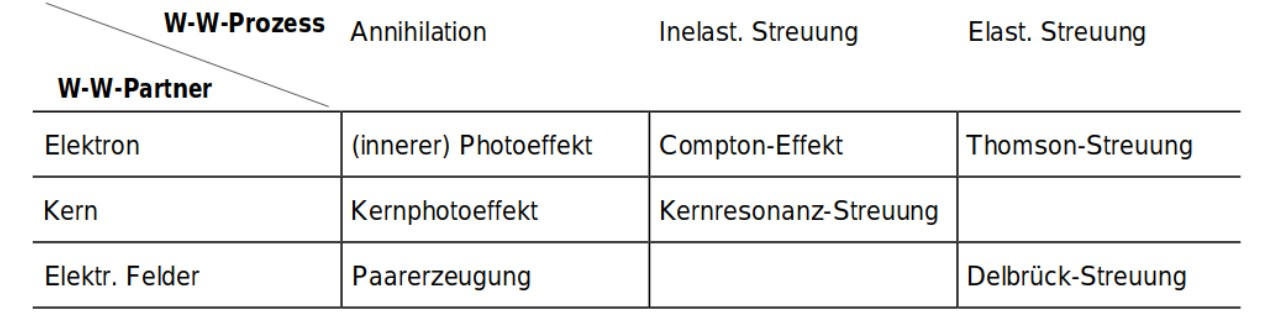
\includegraphics[scale=0.3]{content/WW.jpg}
  \caption{Tabelle zum Zusammenhang der Wechselwirkungen von $\gamma$-Quanten mit Materie [1].}
  \label{fig:WW}
\end{figure}

Für diesen Versuch entscheidend sind der innere Photoeffekt, der Compton-Effekt 
und die Paarerzeugung, da diese hauptsächlich bei Energien von $\SI{10}{\kilo\eV}$ bis 
$\SI{10}{\mega\eV}$ auftreten.\\

Beim inneren Photoeffekt findet ein Annihilationsporzess statt, d.h. dass 
$\gamma$-Quant wird bei der Wechselwirkung mit einem Hüllenelektron vernichtet. Dabei 
löst es dieses aus seiner Bindung und überträgt ihm seine gesamte Energie. Dafür 
muss zunächst die Bindungsenergie des Elektrons überwunden werden. Demnach gibt es 
eine untere Energiegrenze für das Photon, ab der der Photoeffekt überhaupt erst 
auftreten kann. Die kinetische Energie des freigewordenen Elektrons $E_\text{e}$ ist 
dann durch 

\begin{equation*}
E_\text{e} = h\nu -E_\text{B}
\end{equation*}

gegeben. Das Produkt $h\nu$ ist dabei die Photonenergie und $E_\text{B}$ die 
Bindungsenergie des Elektrons. Der Photoeffekt ist dabei schon ab mittleren 
Quantenenergien vernachlässigbar.\\
Beim Compton-Effekt wird das Photon an einem freien Elektron gestreut. Dadurch 
erfährt das $\gamma$-Quant eine Energie- und Richtungsänderung, es gibt dabei 
aber niemals seine gesamte Energie ab. Nach dem Streuprozess ist der $\gamma$-Strahl 
nicht mehr gebündelt und verliert so an Intensität. In Abbidlung \ref{fig:com} findet sich eine 
anschauliche Skizze zu diesem Prozess.

\begin{figure}
  \centering
  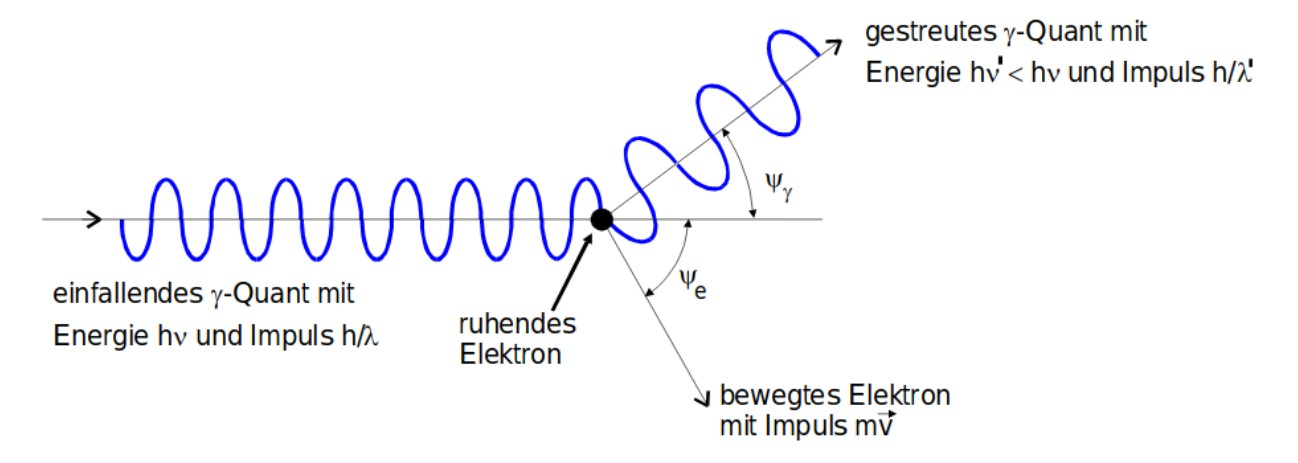
\includegraphics[scale=0.3]{content/com.jpg}
  \caption{Schematische Darstellung des Compton-Effekts [1].}
  \label{fig:com}
\end{figure}

Der Wirkungsquerschnitt des Compton-Effekts $\sigma_\text{com}$ wurde von Klein
und Nishina bestimmt und ist durch 

\begin{equation*}
\sigma_\text{com} = 2\pi r_\text{e}^2 \left(\frac{1+\epsilon}{\epsilon^2}\left[\frac{2(1+\epsilon)}{1+2\epsilon}-\frac{1}{\epsilon}\ln{(1+2\epsilon)}\right]+\frac{1}{2\epsilon}\ln{(1+2\epsilon)}-\frac{1+3\epsilon}{(1+2\epsilon)²}\right)
\label{eqn:sigmacompton}
\end{equation*}

gegeben. $\epsilon$ gibt dabei das Verhältnis zwischen Quantenenergie $E_\text{\gamma}$
und der Ruheenergie des Elektrons 

\begin{equation*}
\epsilon = \frac{E_\text{\gamma}}{m_0 c²}
\end{equation*}

an. $r_\text{e}$ bezeichnet außerdem den klassischen Elektronenradius 
$r_\text{e}=\SI{2.82e-15}{\meter}$ [1].
Für den Compton-Absorptionskoeffizienten $\mu_\text{Compton}$ folgt dann

\begin{equation}
    \label{eqn:mucompton}
    \mu =n \cdot \sigma = \frac{Z N_\text{A} \rho }{M} \cdot \sigma_\text{Compton} \;.
\end{equation}
\\

Die Paarerzeugung tritt dann auf, wenn die Energie der Photonen mehr als doppelt so 
groß ist, als die Ruhemasse des Elektrons ($\SI{1.02}{\mega\eV}$). Das $\gamma$-Quant 
wird dabei annhiliert und es entstehen ein Elektron und ein Positron. Da Impulserhaltung
gelten muss, wird der überschüssige Impuls an die Atomkerne des Absorbermaterials oder 
einen anderen Stoßpartner abgegeben. In Abbildung \ref{fig:ger} sind die Kurvenverläufe 
der Absorptionskoeffizient getrennt nach den verschiedenen Wechselwirkungen in 
Abhängigkeit zu der Energie am Beispiel von Germanium aufgetragen. Die Totalkurve
fügt die Absorptionskoeffizient der einzelnen Wechselwirkungen zusammen.

\begin{figure}
  \centering
  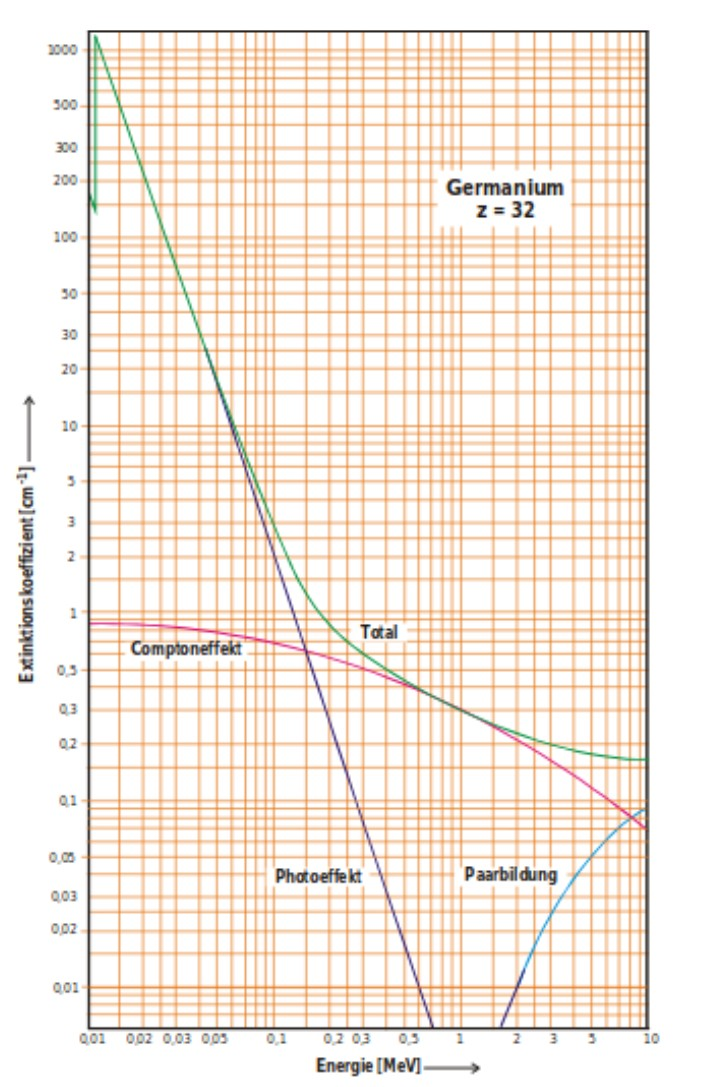
\includegraphics[scale=0.3]{content/ger.jpg}
  \caption{Beispielhafte Kurvenverläufe der Absorptionskoeffizient in Abhängigkeit von der Energie (Germaniumquelle)[1].}
  \label{fig:ger}
\end{figure}

\subsection{\texorpdfstring{$\beta$-Strahlung}{Beta-Strahlung}}

Bei $\beta$-Starhlung handelt es sich um schnelle Elektronen positiver oder 
negativer Ladung. Sie entstehen beim Zerfall von instabilen Atomkernen nach 
der Gleichung 

\begin{equation*}
n \rightarrow p + \beta^{-} + \bar{v_\text{e}}.
\end{equation*}

Entweder es wird aus einem Neutron ein Proton, ein Elektron und ein Antineutrino
erzeugt, oder aus einem Proton ein Neutron, ein Elektron und ein Neutrino. Wir betrachten
im Folgenden den ersten Prozess. Die Energie, die bei diesem Prozess frei wird verteilt
sich statistisch auf das Neutrino und das Elektron. Dies hat zur Folge, dass 
$\beta$-Strahlung ein kontinuierliches Spektrum, statt einem Linienspektrum besitzt.
Die maximale Energie, die das Elektron bei diesem Prozess erhalten kann, ist die
gesamte Energie, die bei dem Zerfall frei wird. \\
$\beta$-Strahlung erfährt eine Vielzahl von Wechselwirkung, wenn sie eine 
Materieschicht durchdringt. Dies liegt hauptsächlich an der Ladung und der 
geringen Masse der $\beta$-Teilchen.\\
Es treten drei wichtige Effekt auf: Die Rutherford-Streuung, inelastische 
Streuung am Atomkern und eine solche an den Elektronen des Absorbermaterials.\\
Bei der Rutherford-Streuung treten elastische Streuungen an Atomkernen des 
Absorbermaterials auf. Hierbei werden die Elektronen im Coulombfeld der Atomkerne
im Absorber in verschiedene Richtungen abgelenkt, was eine Intensitätsabnahme des
$\beta$-Strahls zur Folge hat. Außerdem wird die Bahn der $\beta$-Teilchen 
verlängert, sodass sie größer als ihre Reichweite wird. Ergebnis ist eine höhrere
Wahrscheinlichkeit weiterer Stoßprozesse. Bei dieser Streuung wird die Richtung
der $\beta$-Teilchen zwar stark beeinflusst, die Energieabnahme ist allerdings 
relativ gering. \\
Die inelastische Streuung an Atomkernen des Absorbermaterials erfolgt durch eine 
Beschleunigung der Elektronen im Coulombfeld des Atomkerns. Dabei tritt 
Bremsstrahlung auf, da sie Energie in Form von elektromagnetischer 
Strahlung abgeben und somit gebremst werden. Der Wirkungsquerschnitt
dieses Prozesses ist durch 

\begin{equation*}
\sigma_\text{Br} = \alpha r_\text{e}^2 z^2
\end{equation*}

gegeben. Die Konstante $\alpha$ steht für die Sommerfeldsche Feinstrukturkonstante.\\

Der letzte hier zu nennende Effekt resultiert aus einer inelastischen Streuung 
der $\beta$-Teilchen an den Elektronen im Absorbermaterial. Dabei ioniersieren 
sie das Material und regen es an. Da die Strahlung dafür nur einen kleinen Teil 
ihrer Energie aufwenden muss, ist ein einzelnes Teilchen dazu fähig, viele 
Absorberatome zu ionisieren und anzuregen. Der Energieverlust pro Absorberschichtdicke
wird durch 

\begin{equation*}
\frac{\symup{d}E}{\symup{d}x} \approx \frac{2\pi r_\text{e}^2}{E_\text{\beta}} \frac{N_\text{A}\rho}{M} z \ln{\left(\frac{E_\text{\beta}}{I}\right)}
\end{equation*}

dargestellt.\\

Für die Absorptionskurve des natürlichen $\beta$-Strahlers gilt analog zur 
Absorptionskurve von $\gamma$-Strahlung ein expontenieller Abfall. Für Schichtdicken, 
die etwa der maximalen Reichweite entsprechen, gilt das expontenielle
Absorptionsgesetz nicht mehr. Im Bereich hinter der maximalen Reichweite wird 
die gemessene Strahlung nicht mehr durch $\beta$-Strahlung hervorgerufen, 
sondern nur noch durch Bremsstrahlung oder kosmische Hintergundstrahlung. 
In Abbildung \ref{fig:kurve} ist eine Absorptionskurve eines $\beta$-Strahlers dargestellt.

\begin{figure}
  \centering
  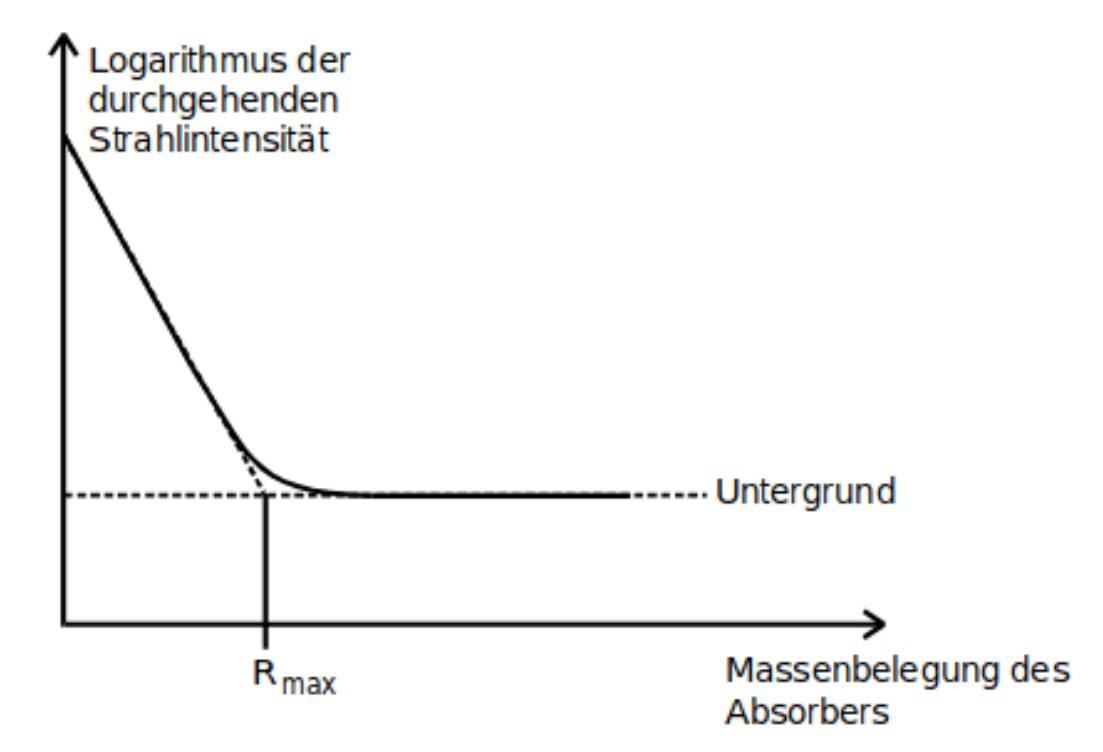
\includegraphics[scale=0.3]{content/kurve.jpg}
  \caption{Typische Absorptionskurve eines $\beta$-Strahlers [1].}
  \label{fig:kurve}
\end{figure}

Aufgetragen ist die logarithmierte Strahlungsintensität gegen die Massenbelegung
$R$ des Absorbers. Diese Größe wird durch 

\begin{equation*}
R = \rho D
\end{equation*}

bestimmt. Die im gesamten Zerfall freiwerdende Energie wird als $E_\text{max}$
bezeichnet. Aus der maximalen Massenbelegung $R_\text{max}$ kann $E_\text{max}$
durch folgende empirisch bestimmte Beziehung errechnet werden

\begin{equation*}
E_\text{max} = \num{1.92}\sqrt{R_\text{max}^2+\num{0.22}R_\text{max}}[\symup{MeV}].
\label{eqn:Emax}
\end{equation*}